%% shaderous: Shaderous: A Browser-based Hydrodynamics Code for Physics Research and Teaching
%% AAS Journals (ApJ, ApJL, ApJS, AJ, PSJ, RNAAS): AASTeX 7.0.1, aastex701.cls.
%% One source, two typesettings, each built by a three-line wrapper that sets \papermode:
%%   submit.tex   -> submit.pdf    single column, easy to referee and to read on screen
%%   preprint.tex -> preprint.pdf  two columns, close to the published article; this goes to arXiv
%% Build both:  cd paper && latexmk -pdf
%% arXiv:       python util/arxiv_zip.py
\providecommand{\papermode}{submit}
\newif\iftwocol
\def\pmpreprint{preprint}\edef\pmgiven{\papermode}
\ifx\pmpreprint\pmgiven \twocoltrue \fi
\iftwocol
  \documentclass[twocolumn]{aastex701}
\else
  \documentclass{aastex701}
\fi

\usepackage{amsmath}
% Column figures: at the column's width in two columns; in one, where the column is the whole
% text width, no taller than this, so that the stacked panels fit on a page.
\iftwocol \newcommand{\colfigheight}{\textheight} \else \newcommand{\colfigheight}{0.42\textheight} \fi
\usepackage{xcolor}
\usepackage{booktabs}

% Paper-wide macros, the ADS journal abbreviations, and the theorem environments.
%% Paper-wide macros. main.tex \inputs this after the class and its packages, so it works
%% unchanged under every journal in templates/journals/.
%%
%% Rules (.cursor/rules/abstract.mdc): none of these may appear in \title or the abstract,
%% which are pasted into arXiv and journal forms as plain text. util/check_abstract.py
%% rejects any command defined here that shows up there.
%%
%% Use \providecommand for anything a class may already define, so the class version wins.

%% ---------------------------------------------------------------- provisional text
% Placeholder or provisional text is set in red so it cannot be mistaken for a result.
% util/check_style.py lists every \todo left in the manuscript.
\providecommand{\todo}[1]{\textcolor{red}{#1}}
% A framed box that stands in for a figure not yet drawn: height, then what it will show.
\providecommand{\figplaceholder}[2]{\fbox{\parbox[c][#1][c]{0.92\linewidth}{\centering\todo{Placeholder. #2}}}}

%% ---------------------------------------------------------------- portable back matter
% AASTeX and REVTeX define these; the other classes get plain equivalents, so the body
% can use them under any journal.
\ifdefined\acknowledgments\else
  \newenvironment{acknowledgments}{\section*{Acknowledgments}}{}
\fi
\providecommand{\software}[1]{\par\medskip\noindent\textit{Software:} #1\par}
\providecommand{\facilities}[1]{\par\medskip\noindent\textit{Facilities:} #1\par}

%% ---------------------------------------------------------------- theorem environments
% amsart loads amsthm; the astronomy classes do not. Numbered within sections.
% elsarticle defines \openbox and mnras defines a proof environment, both of which amsthm
% would define again; clear them so amsthm's versions are used everywhere.
\ifdefined\theoremstyle\else
  \ifdefined\openbox\let\openbox\relax\fi
  \ifdefined\proof\let\proof\relax\let\endproof\relax\fi
  \usepackage{amsthm}
\fi
\ifdefined\theorem\else
  \theoremstyle{plain}
  \newtheorem{theorem}{Theorem}[section]
  \newtheorem{lemma}[theorem]{Lemma}
  \newtheorem{proposition}[theorem]{Proposition}
  \newtheorem{corollary}[theorem]{Corollary}
  \theoremstyle{definition}
  \newtheorem{definition}[theorem]{Definition}
  \newtheorem{example}[theorem]{Example}
  \theoremstyle{remark}
  \newtheorem{remark}[theorem]{Remark}
\fi

%% ---------------------------------------------------------------- mathematics
% Upright differential with the right spacing: \int f(x)\dd x.
\providecommand{\dd}{\mathop{}\!\mathrm{d}}
\providecommand{\R}{\mathbb{R}}
\providecommand{\C}{\mathbb{C}}
\providecommand{\Z}{\mathbb{Z}}
\providecommand{\N}{\mathbb{N}}
\providecommand{\Q}{\mathbb{Q}}
\providecommand{\E}{\mathbb{E}}
\providecommand{\abs}[1]{\left\lvert #1\right\rvert}
\providecommand{\norm}[1]{\left\lVert #1\right\rVert}
\providecommand{\Var}{\operatorname{Var}}
\providecommand{\Cov}{\operatorname{Cov}}
\providecommand{\sgn}{\operatorname{sgn}}
\providecommand{\bigO}{\mathcal{O}}

%% ---------------------------------------------------------------- astronomy
\providecommand{\Msun}{\ensuremath{M_\odot}}
\providecommand{\Rsun}{\ensuremath{R_\odot}}
\providecommand{\Lsun}{\ensuremath{L_\odot}}
\providecommand{\Mearth}{\ensuremath{M_\oplus}}
\providecommand{\Rearth}{\ensuremath{R_\oplus}}
\providecommand{\Mjup}{\ensuremath{M_{\rm J}}}
\providecommand{\Rjup}{\ensuremath{R_{\rm J}}}
\providecommand{\kms}{\ensuremath{\mathrm{km\,s^{-1}}}}
\providecommand{\Hnot}{\ensuremath{H_0}}

%% ---------------------------------------------------------------- journal abbreviations
% The macros that ADS writes into BibTeX. AASTeX, mnras and aa define them already;
% elsarticle, REVTeX and amsart do not.
\providecommand{\aj}{AJ}
\providecommand{\actaa}{Acta Astron.}
\providecommand{\araa}{ARA\&A}
\providecommand{\apj}{ApJ}
\providecommand{\apjl}{ApJL}
\providecommand{\apjs}{ApJS}
\providecommand{\ao}{Appl.\ Opt.}
\providecommand{\apss}{Ap\&SS}
\providecommand{\aap}{A\&A}
\providecommand{\aapr}{A\&A~Rev.}
\providecommand{\aaps}{A\&AS}
\providecommand{\azh}{AZh}
\providecommand{\baas}{BAAS}
\providecommand{\icarus}{Icarus}
\providecommand{\jcap}{JCAP}
\providecommand{\jrasc}{JRASC}
\providecommand{\memras}{MmRAS}
\providecommand{\mnras}{MNRAS}
\providecommand{\na}{New Astron.}
\providecommand{\nar}{New Astron.\ Rev.}
\providecommand{\pra}{Phys.\ Rev.\ A}
\providecommand{\prb}{Phys.\ Rev.\ B}
\providecommand{\prc}{Phys.\ Rev.\ C}
\providecommand{\prd}{Phys.\ Rev.\ D}
\providecommand{\pre}{Phys.\ Rev.\ E}
\providecommand{\prl}{Phys.\ Rev.\ Lett.}
\providecommand{\pasa}{PASA}
\providecommand{\pasp}{PASP}
\providecommand{\pasj}{PASJ}
\providecommand{\psj}{PSJ}
\providecommand{\qjras}{QJRAS}
\providecommand{\skytel}{S\&T}
\providecommand{\solphys}{Sol.\ Phys.}
\providecommand{\sovast}{Soviet Ast.}
\providecommand{\ssr}{Space Sci.\ Rev.}
\providecommand{\zap}{ZAp}
\providecommand{\nat}{Nature}
\providecommand{\natas}{Nature Astron.}
\providecommand{\iaucirc}{IAU~Circ.}
\providecommand{\aplett}{Astrophys.\ Lett.}
\providecommand{\apspr}{Astrophys.\ Space Phys.\ Res.}
\providecommand{\grl}{Geophys.\ Res.\ Lett.}
\providecommand{\jgr}{J.\ Geophys.\ Res.}
\providecommand{\jqsrt}{JQSRT}
\providecommand{\physrep}{Phys.\ Rep.}
\providecommand{\physscr}{Phys.\ Scr.}
\providecommand{\planss}{Planet.\ Space Sci.}
\providecommand{\procspie}{Proc.\ SPIE}

%% ---------------------------------------------------------------- this paper
% Add the paper's own macros below. Keep them few: a reader should not need a glossary.

% A wrapped table cell of a given width. Used instead of p{} columns, which aastex701
% breaks under some MiKTeX installations ("Extra \or").
\providecommand{\tabpar}[2]{\parbox[t]{#1}{\raggedright #2\strut}}


% Keep short inline math on one line in the single-column layout. A long formula that
% must break is wrapped as {\relpenalty=200 $...$}. Two columns keep TeX's defaults.
\iftwocol
  \emergencystretch=3em
\else
  \relpenalty=10000
  \binoppenalty=10000
  \emergencystretch=1em
\fi

\shorttitle{Shaderous}
\shortauthors{Guillochon}

\begin{document}

\title{Shaderous: A Browser-based Hydrodynamics Code for Physics Research and Teaching}

\author{James Guillochon}
\affiliation{Independent Researcher}
\email{guillochon@gmail.com}

% The abstract is primitive TeX on purpose: arXiv and the journal take it as pasted text.
\begin{abstract}
Shaderous is a three-dimensional code for compressible gas dynamics that runs entirely in WebGPU compute shaders inside a web browser on any vendor's graphics processor. We demonstrate it on astrophysical problems, which use every part of the solver at once. It combines an unsplit MUSCL-Hancock scheme and HLLC fluxes with a multigrid Poisson solver, block-structured adaptive mesh refinement with per-block timesteps, point masses with sinks, optically thin cooling, viscosity, thermal conduction, and several equations of state. A setup is shared as a link and runs on a student's own laptop or phone, so the code suits teaching. We describe classroom uses for non-major undergraduates, physics and astronomy majors, and graduate students, from watching an instability grow to measuring convergence and changing the solver. Three aspects of the design are, as far as we can find, new. First, no face flux is ever stored. The two cells that share a face compute bit-identical fluxes, so a coarse cell next to a refined region recomputes the fine fluxes instead of keeping a flux register, and a block that steps less often than its neighbor recomputes that neighbor's fluxes from stored states. Mass, momentum and energy are then conserved to round-off on the adaptive mesh. Second, the whole step runs on the GPU: the timestep and the assignment of blocks to time bins are reduced there, and ghost cells are computed as they are loaded rather than exchanged. Third, the code works in single precision throughout and still holds hydrostatic stars and atmospheres in balance, using a well-balanced reconstruction after K\"appeli \& Mishra (2014) and initial states settled against the grid's own potential. An isothermal column whose density falls by a factor of nine million stays below Mach $4\times10^{-5}$ after a sound crossing, against 0.35 without. A suite of 36 validation tests runs on the reader's own GPU.
\end{abstract}

\keywords{Hydrodynamics --- Hydrodynamical simulations --- Computational methods --- GPU computing --- Astronomy software}

%% ---- BODY ----
%% Everything between the BODY markers is journal-independent: util/new_paper.py --switch
%% carries it to another journal class unchanged. Keep class-specific markup out of it.

\section{Introduction}
\label{sec:intro}

Grid codes for astrophysical gas dynamics, such as FLASH \citep{Fryxell2000}, RAMSES \citep{Teyssier2002} and Athena++ \citep{Stone2020}, are large native programs. A user compiles them against a compiler, an MPI library and, on graphics processors, a vendor toolchain, then runs them on a workstation or a cluster and inspects the output afterward. That workflow suits production science. It is a poor fit for teaching, for exploring a problem before committing to a production run, and for handing a colleague a result that they can reproduce and modify in a minute.

Graphics processors entered numerical gas dynamics through their graphics interfaces. Before CUDA, solvers were written as fragment programs that read and wrote textures: linear algebra and multigrid \citep{Bolz2003, Goodnight2003, Kruger2003}, incompressible cloud dynamics \citep{Harris2003}, and the compressible Euler equations with high-resolution finite-volume schemes in two and three dimensions \citep{Hagen2006}. \citet{Owens2007} surveyed that period. General-purpose toolchains then replaced the graphics route, and astrophysics gained a generation of GPU codes, among them GAMER \citep{Schive2010, Schive2018}, the adaptive solver of \citet{Wang2010}, the Euler solver of \citet{Kestener2010}, Cholla \citep{Schneider2015}, FARGO3D \citep{BenitezLlambay2016}, Astaroth \citep{Pekkila2017}, K-Athena \citep{Grete2021}, Quokka \citep{Wibking2022}, Idefix \citep{Lesur2023}, Kratos \citep{Wang2025}, AthenaK \citep{Stone2026}, AGILE \citep{Porth2026} and RAMSES-GPU \citep{Teyssier2026}. These codes are fast and scale to many devices, but each is a native application built with CUDA, HIP or a portability layer.

WebGPU, a graphics and compute interface that browsers now ship, brings compute shaders to every desktop and many phones without an installation step. Its shading language, WGSL, compiles to whatever the local driver accepts. Simulators that use the GPU from a browser exist for reaction-diffusion and cardiac models \citep{Kaboudian2019} and for the Gross-Pitaevskii equation \citep{Baggaley2026}, but we found none that solves the compressible Euler equations with shocks, self-gravity or adaptive refinement (Section~\ref{sec:prior}).

This paper describes Shaderous, a code that does. All fluid and gravity computation runs in WGSL compute shaders, and the code runs at a web address. Nothing in the scheme is specific to astrophysics. It solves the compressible Euler equations with optional gravity, diffusion, heating and cooling, and serves the same purpose in a course on fluid dynamics or for a problem in another field. We demonstrate it on astrophysical problems because they exercise every part of the code at once: strong shocks, self-gravity, stars that must stay in hydrostatic balance, point masses that accrete, cooling, and equations of state as far from an ideal gas as degenerate electrons. The physics is conventional and we credit its sources throughout. What is new is how the scheme is mapped onto an interface designed for graphics. WebGPU forbids a pass from reading and writing the same four-channel floating-point texture, has no double precision, limits the number of storage bindings, and returns data to the CPU only asynchronously. We turned each restriction into a design choice. The result is a code that conserves to round-off on an adaptive mesh without storing a single face flux, that never exchanges ghost cells, that keeps every step on the GPU, and that keeps hydrostatic objects in balance in single precision.

Section~\ref{sec:prior} compares Shaderous with earlier work. Section~\ref{sec:webgpu} describes the constraints of WebGPU and the data layout that follows from them. Section~\ref{sec:hydro} gives the hydrodynamic scheme, Section~\ref{sec:conservation} the flux evaluation that conserves without stored fluxes, Section~\ref{sec:amr} the adaptive mesh and its local timesteps, and Section~\ref{sec:gravity} gravity, point masses and sinks. Section~\ref{sec:interface} describes the interface, the file format and the interfaces for scripts, Section~\ref{sec:education} the uses of the code in teaching, Section~\ref{sec:validation} the validation suite, and Section~\ref{sec:performance} performance. Section~\ref{sec:discussion} discusses limitations.

\section{Relation to earlier work}
\label{sec:prior}

We searched for earlier codes in three literatures (see \texttt{research/prior-art.md} in the paper repository): general-purpose computation in graphics shaders, GPU codes for astrophysical fluids, and scientific simulators that run in a browser.

The shader-era solvers are the closest in spirit. \citet{Hagen2006} solved the compressible Euler equations on uniform grids in fragment programs, and \citet{Goodnight2003} and \citet{Bolz2003} ran multigrid in the same way. Adaptive data structures in textures also came from computer graphics: \citet{Lefohn2006} built page tables and octrees in textures for random access on the GPU. Shaderous uses compute shaders rather than fragment programs, but it inherits the same model of state held in textures and updated by one invocation per cell. It adds what those solvers did not have: self-gravity, adaptive refinement with conservative coupling between levels, local timesteps, and the physics of astrophysical problems.

Among GPU codes for astrophysics, GAMER \citep{Schive2010, Schive2018} and the code of \citet{Wang2010} are the closest in structure: both refine in fixed-size patches or blocks, as Shaderous does. They follow \citet{Berger1989} in correcting the coarse side of a refinement boundary with fluxes stored from the fine side. Shaderous stores no fluxes at all (Section~\ref{sec:conservation}).

The browser simulators of \citet{Kaboudian2019} and \citet{Baggaley2026} show that interactive computing on the GPU through WebGL and WebGPU is practical. They solve reaction-diffusion and Schr\"odinger-type equations on uniform grids, where no conservation law has to hold across a shock or a refinement boundary.

\section{Constraints of WebGPU and the data layout}
\label{sec:webgpu}

Four properties of WebGPU shaped the code. Each is a property of the interface, not of the hardware.

\emph{No read-write access to four-channel floating-point textures.} A compute pass can write an \texttt{rgba32float} texture only as a write-only storage texture. Every update therefore reads one copy of the state and writes another. Single-channel \texttt{r32float} textures can be read and written in one pass, which the red-black smoother of the Poisson solver uses.

\emph{Limited storage buffers.} The default limits allow few storage buffers per shader stage and cap a single binding at 128~MB. We hold the state in 3D textures instead: density and momentum in one \texttt{rgba32float} texture, and total energy, internal energy and a passive scalar in a second. We measured the same flux stencil on storage buffers and found it about 1.4 times slower than on textures.

\emph{No double precision.} WGSL has no 64-bit floating-point type. Every quantity is a 32-bit float, and the scheme has to hold hydrostatic balance and track internal energy in fast flows at that precision (Sections~\ref{sec:robustness} and~\ref{sec:wellbalanced}).

\emph{Asynchronous readback.} Data return to the CPU only through a mapped buffer, some frames later. A code that reads the timestep back before every step would stall. Shaderous computes the timestep on the GPU, writes it to a small buffer, and lets the following passes read it there. The CPU reads diagnostics and refinement indicators without waiting for them.

WGSL also has no dynamic dispatch. A small preprocessor assembles each shader from modules: the equation of state, the Riemann solver, the slope limiter, the cooling function and the diffusive fluxes in use are chosen when the shaders are built, and changing one rebuilds the affected pipelines. A module that is switched off maps to a stub, so a run without species, cooling or diffusion pays nothing for them.

Reductions run in stages. The timestep, the diagnostics and the refinement indicators all use them. Each stage folds blocks of $4^3$ records from the stage before, so sums are formed hierarchically, which limits the round-off of single precision. Maxima of non-negative values are accumulated with an atomic maximum on their bit patterns, which order the same way as the floating-point values.

No browser reports how much memory its GPU has, and a phone that runs out kills the page before WebGPU reports an error. Shaderous therefore guesses a memory budget from what the browser does report: 2.5~GB for a discrete desktop GPU, 2~GB where the GPU shares the system's memory, and 1~GB on a phone. The user can change it. Before each large allocation the page leaves a note in the browser's local storage. A note that is still there when the page next loads means that the page crashed holding that much memory, and the budget is then lowered below it for good.

\section{Hydrodynamics}
\label{sec:hydro}

Shaderous solves the Euler equations with gravity,
\begin{equation}
\begin{aligned}
\partial_t \rho + \nabla\cdot(\rho\mathbf{v}) &= 0,\\
\partial_t (\rho\mathbf{v}) + \nabla\cdot(\rho\mathbf{v}\mathbf{v} + p\,\mathsf{I}) &= -\rho\nabla\Phi,\\
\partial_t E + \nabla\cdot\bigl[(E + p)\mathbf{v}\bigr] &= -\rho\mathbf{v}\cdot\nabla\Phi + \mathcal{H} - \mathcal{C},
\end{aligned}
\label{eq:euler}
\end{equation}
where $\rho$ is the density, $\mathbf{v}$ the velocity, $p$ the pressure, $E$ the total energy density, $\Phi$ the gravitational potential, $\mathsf{I}$ the identity, and $\mathcal{H}$ and $\mathcal{C}$ the heating and cooling rates per unit volume. A passive scalar is advected with the gas, and the internal energy density $e$ is evolved alongside $E$ (Section~\ref{sec:robustness}).

\subsection{Scheme}
\label{sec:scheme}

The scheme is an unsplit MUSCL-Hancock method \citep{vanLeer1979}, in the form given by \citet{Toro2009}. A predictor pass advances each cell half a step from its own reconstructed slopes. An update pass then reconstructs face states from the half-step values, solves a Riemann problem at each of the cell's six faces, and applies the flux differences and the gravitational source. With the passes that compute the signal speed and reduce the timestep, a step is four passes. On the uniform grid no primitive variables are stored: the predictor and the update convert the conserved state as they load it, because the flux update is limited by texture fetches (with all of its arithmetic removed, it still takes 85 percent as long) and a pass that only rewrites the state costs more than repeating the conversion. Figure~\ref{fig:hydro} shows the accuracy of the scheme on a shock tube, a blast and a smooth flow.

\begin{figure*}[t]
\centering
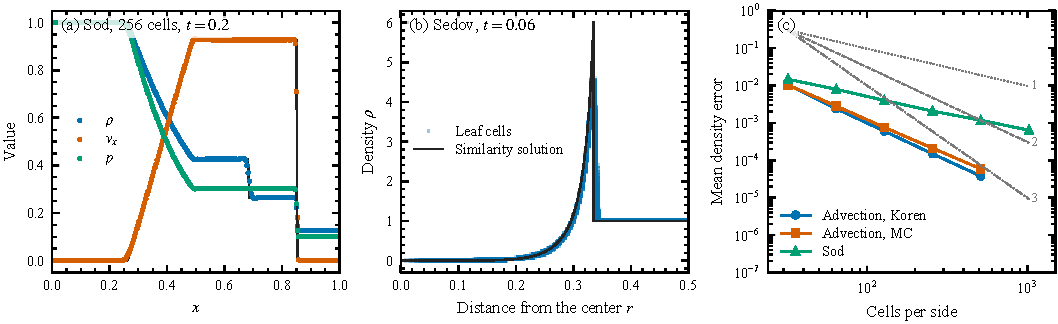
\includegraphics[width=\textwidth]{figures/hydro.pdf}
\caption{Accuracy of the hydrodynamics. (a)~Density, velocity and pressure of the Sod shock tube at $t = 0.2$ along the middle row of a $256^2$ grid (points), and the exact solution (lines). (b)~Density against distance from the center for the leaf cells of a three-dimensional Sedov blast on the adaptive mesh (finest resolution 256 cells, three levels) at $t = 0.06$, every 33rd of the 6.5 million cells (points), and the similarity solution (line). (c)~Mean density error against the number of cells per side for a Gaussian advected once around the periodic box along a diagonal, with the default limiter of \citet{Koren1993} and the monotonized central limiter, and for the Sod tube; gray lines show first-, second- and third-order convergence.}
\label{fig:hydro}
\end{figure*}

The timestep is the smallest of three limits: $C\,\Delta x/\max_i(|v_i| + c_{\rm s})$, $C\sqrt{\Delta x/\max|\mathbf{g}|}$, and the limit of each pair of point masses (Section~\ref{sec:sinks}). Here $C = 0.8$ is the CFL number, $\Delta x$ the cell size, $v_i$ a component of the velocity, $c_{\rm s}$ the sound speed, and $\mathbf{g}$ the gravitational acceleration. The maxima run over all cells. The step is also shortened so that it ends exactly on the next output time. Viscosity and conduction add a signal speed (Section~\ref{sec:diffusion}); cooling does not limit the step (Section~\ref{sec:eos}).

The fluxes come from the HLLC solver of \citet{Toro1994}, the HLL solver of \citet{Harten1983}, or a low-Mach variant of HLLC. Wave speeds are the estimates of \citet{Davis1988}, {\relpenalty=200 $S_{\rm L} = \min(u_{\rm L} - c_{\rm L},\, u_{\rm R} - c_{\rm R})$} and {\relpenalty=200 $S_{\rm R} = \max(u_{\rm L} + c_{\rm L},\, u_{\rm R} + c_{\rm R})$}. Here $u$ is the velocity normal to the face, $c$ the sound speed, and L and R denote the two sides of the face. These estimates need only the pressure and the sound speed on each side, so the solvers do not depend on the equation of state. Barotropic gas uses HLL, since it has no contact wave for HLLC to resolve.

The low-Mach variant follows \citet{Thornber2008}: the velocity jump handed to HLLC is scaled by the local Mach number, so that slow flow is not damped at a rate set by the sound speed:
\begin{equation*}
\begin{aligned}
\mathbf{v}_{\rm L,R} &\rightarrow \tfrac{1}{2}(\mathbf{v}_{\rm L} + \mathbf{v}_{\rm R}) \pm \tfrac{z}{2}(\mathbf{v}_{\rm L} - \mathbf{v}_{\rm R}),\\
z &= \min\bigl[1,\ \max\bigl(z_{\rm min},\ |\mathbf{v}_{\rm L}|/c_{\rm L},\ |\mathbf{v}_{\rm R}|/c_{\rm R}\bigr)\bigr].
\end{aligned}
\end{equation*}
We set the floor $z_{\rm min}$ to 0.3. With one predictor and one update and the unlimited third-order reconstruction below, the scheme relies on some of the solver's damping, and a Gresho vortex \citep{Gresho1990} at Mach 0.01 gains kinetic energy without bound for a floor of 0.1 or less. With the floor at 0.3, that vortex on $64 \times 64$ cells loses 6 percent of its kinetic energy in two time units, against 15 percent with plain HLLC. Scaling the acoustic wave speeds instead, as \citet{Fleischmann2020} do, also removes the damping of pressure jumps and was unstable in this scheme at Mach 0.03.

\subsection{Reconstruction}
\label{sec:recon}

The default reconstruction gives each face the value of the parabola through the cell and its two neighbors, which is third-order accurate on the three-cell stencil that a slope limiter already uses. The face value is $q_{\rm c} + (\delta_{\rm far} + 2\delta_{\rm near})/6$, where $q_{\rm c}$ is the value in the cell, $\delta_{\rm near}$ the difference to the neighbor on the side of the face, and $\delta_{\rm far}$ the difference to the neighbor on the other side. A three-cell limiter cannot tell a smooth extremum from a jump and flattens both. Following the idea of \citet{Cada2009}, we apply a limiter only where a quantity changes by more than 1 percent of its natural scale across a cell: the density, the pressure, or the sound speed for the velocities. Calling that scale $Q$, the face value blends from the unlimited value to the limited one as $(\delta_{\rm near}^2 + \delta_{\rm far}^2)/(0.01\,Q)^2$ rises from 0.5 to 1.5. The limiter is that of \citet{Koren1993} with the bounds of the monotonized central limiter \citep{vanLeer1977}. A smooth peak then keeps its height: the largest error in the advection test is 2.5 to 5 times smaller than with the monotonized central limiter (Figure~\ref{fig:hydro}c). Kinks and jumps smaller than 1 percent go unlimited, and shock-tube errors are a few percent higher on axis-aligned tubes. The monotonized central, \citet{vanLeer1974} and minmod \citep{Roe1986} limiters remain available.

\subsection{Robustness in single precision}
\label{sec:robustness}

Single precision loses the pressure of gas whose kinetic energy dominates its total energy. We evolve the internal energy alongside the total energy and use it where the kinetic energy dominates, after the dual-energy formalism of \citet{Bryan1995}. The internal energy that we evolve replaces the difference of the total and kinetic energies wherever that difference is below $10^{-3}$ of the total energy, or below the least internal energy that the equation of state allows. Where we use it, we rebuild the total energy from it, except in degenerate gas. There we keep the total energy as the conservative update left it and take only the pressure from the internal energy, because a degenerate gas has a pressure, at least that of its cold electrons, even where the total energy minus the kinetic energy is negative. In a collision of two white dwarfs that difference turns negative in the cell ahead of each strong shock. Rebuilding the total energy there added 2.3 percent to it at the moment of greatest compression. Keeping it leaves a change of 0.6 percent through the collision. A face state with a nonpositive density or pressure drops its cell to first order for that step. Next to a cell flagged by a pressure-jump shock detector, the flux blends from HLLC toward HLL, which suppresses the carbuncle instability \citep{Quirk1994}. The detector flags a cell where the flow converges and the pressures of its two neighbors along some axis differ by more than half of the smaller one. It measures that difference against hydrostatic balance (Section~\ref{sec:wellbalanced}). Density and pressure floors, by default $10^{-10}$ and $10^{-14}$ in code units, catch what remains, and the number of floored cells is reported as a diagnostic.

\subsection{Well-balanced reconstruction}
\label{sec:wellbalanced}

In hydrostatic balance the pressure is not smooth across a stratified cell; its balance with gravity is. Following \citet{Kappeli2014}, what is limited and reconstructed is each neighbor's deviation from that balance,
\begin{equation}
\delta p = (p_{\rm n} - p_{\rm c}) + \tfrac{1}{2}(\rho_{\rm c} + \rho_{\rm n})(\Phi_{\rm n} - \Phi_{\rm c}),
\label{eq:wb}
\end{equation}
where the subscripts c and n denote the cell and its neighbor. The balanced part of the step to the face, $-\rho_{\rm c}\,\Delta\Phi$, is added back unlimited. Where the cells obey the trapezoid rule of Equation~(\ref{eq:wb}) with $\delta p = 0$, the two cells that share a face agree on its pressure, and a cell's two face pressures differ by exactly the momentum that the gravity kick adds. The state then holds to round-off however steep it is. The shock detector measures pressure jumps against the same balance, so that a steep atmosphere at rest is not flagged as a shock. An isothermal column whose density falls by a factor of $e$ every four cells keeps its largest Mach number at $4 \times 10^{-5}$ after a sound crossing, against 0.35 without the balanced reconstruction (Figure~\ref{fig:balance}a). The background of the Rayleigh-Taylor problem is 240 times quieter, and the error in the growth rate of the Jeans instability is 12 times smaller.


\subsection{Equations of state and cooling}
\label{sec:eos}

Every equation of state implements the same four functions (pressure, sound speed, internal energy from pressure, temperature), so the hydrodynamic passes are independent of it. Shaderous provides an ideal gas, a barotropic gas (isothermal or polytropic), and an ideal gas plus radiation pressure in local thermodynamic equilibrium, whose temperature comes from a Newton iteration with a fixed number of steps. Each WGSL module has a double-precision mirror in TypeScript for testing.

\begin{figure}[t]
\centering
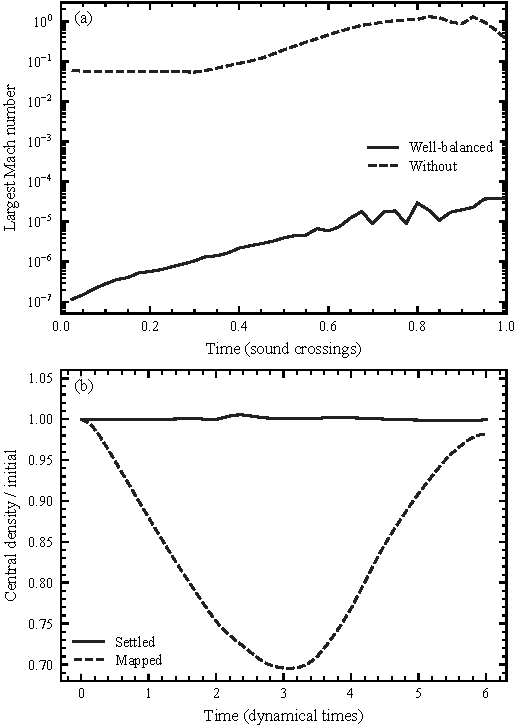
\includegraphics[width=\columnwidth,height=\colfigheight,keepaspectratio]{figures/balance.pdf}
\caption{Hydrostatic balance in single precision. (a)~Largest Mach number in an isothermal column whose density falls by a factor of $e$ every four cells, over one sound crossing, with the well-balanced reconstruction (solid) and without it (dashed). (b)~Central density of a white dwarf of $1\,\Msun$ on the adaptive mesh (finest resolution 256 cells, two levels), settled against the grid's own potential (solid) and mapped from its analytic profile (dashed), relative to its starting value.}
\label{fig:balance}
\end{figure}

Two further equations of state use the composition of the gas, which a problem with physical units gives as a list of species and their mass fractions. The first adds the pressure of fully degenerate electrons at any degree of relativity \citep{Chandrasekhar1935} to an ideal gas and radiation, for white dwarfs. Its density scale follows from the number of electrons per nucleon. Each part is thermodynamically consistent on its own, so the square of the sound speed is the derivative of the degenerate pressure plus $\Gamma_1 p_{\rm th}/\rho$ of the thermal part. Where the Fermi momentum is below half of $m_{\rm e} c$, the pressure and energy of the degenerate gas are summed as series, because their closed forms cancel to nothing in single precision. The second equation of state lets hydrogen ionize in Saha equilibrium \citep{Saha1920}, so that the mean molecular weight and the internal energy, which includes 13.6~eV per ionization, follow the temperature. Its adiabatic index is computed exactly and dips below 1.3 in the ionization zone. Its temperature comes from Newton's method kept inside a bracket.

Optically thin cooling is either a power law in temperature with uniform heating, or the interstellar cooling function of \citet{Koyama2002} with the correction of \citet{VazquezSemadeni2007}. In the second, the internal energy per unit volume changes at the rate $n\Gamma\,[1 - n\Lambda(T)/\Gamma]$, where $n$ is the number density of hydrogen atoms in cm$^{-3}$, $\Gamma$ the heating rate per atom, $T$ the temperature in kelvin, and
\begin{equation*}
\begin{aligned}
\frac{\Lambda(T)}{\Gamma} ={}& 10^{7}\exp\left(\frac{-1.184\times10^{5}}{T + 1000}\right)\\
&+ 1.4\times10^{-2}\sqrt{T}\,\exp\left(\frac{-92}{T}\right).
\end{aligned}
\end{equation*}
Cooling is applied to the internal energy at fixed density at the end of the update, in up to 12 second-order substeps that each change the energy by at most a tenth. A substep that would cross thermal balance stops at the balance point, so cooling times far shorter than the timestep are stable and do not overshoot. The timestep is not shortened for cooling.

\subsection{Viscosity and conduction}
\label{sec:diffusion}

Shaderous can add a viscous stress and a conductive heat flux to Equation~(\ref{eq:euler}). The momentum flux gains $-\boldsymbol{	au}$ and the energy flux gains $-\boldsymbol{	au}\cdot\mathbf{v} + \mathbf{q}$, with
\begin{equation}
\begin{aligned}
\boldsymbol{	au} &= \rho\nu\left[\nabla\mathbf{v} + (\nabla\mathbf{v})^{\rm T} - \tfrac{2}{3}(\nabla\cdot\mathbf{v})\,\mathsf{I}\right],\\
\mathbf{q} &= -\kappa\rho\nabla T,
\end{aligned}
\label{eq:diffusion}
\end{equation}
where $T$ is the temperature, and the kinematic viscosity $\nu$ and the coefficient $\kappa$ are constants. The temperature of an ideal gas with adiabatic index $\gamma$ then diffuses at $(\gamma - 1)\kappa$.

Both fluxes are evaluated explicitly from the state at the start of the step and added to the Riemann flux of each face. Derivatives along the normal of a face are differences of its two cells. Derivatives across it are the mean of the centered differences in the two cells. Because the diffusive terms are part of the face flux, the properties of that flux carry over to them. The two cells that share a face compute the same bits, and the matching of Sections~\ref{sec:reflux} and~\ref{sec:timebins} conserves momentum and energy across refinement boundaries and between blocks on different timesteps. On the adaptive mesh the transverse differences on the rim of a block's face would need edge ghost cells, which Shaderous never computes. Both blocks that share the face use one-sided differences along the rim instead. A face of an obstacle is a wall at rest to which the gas sticks and through which no heat passes. The heat that the stress dissipates is added to the separately evolved internal energy (Section~\ref{sec:robustness}).

The timestep counts diffusion as an additional signal speed of $2.5\,d\,D/\Delta x$, where $d$ is the number of dimensions, $\Delta x$ the cell size, and $D$ the larger of $4\nu/3$ and the thermal diffusivity. The step therefore falls as $\Delta x^2$ where diffusion dominates. There is no implicit solve, so strong diffusion on a fine mesh is slow. Viscosity lengthens the flux update by a factor of 1.6 in two dimensions and 1.8 in three, because the transverse derivatives need the cells diagonally across from the one being updated. Conduction alone adds no measurable time.

\subsection{Species}
\label{sec:species}

A problem can carry any number of species, as mass fractions $X_k$ that sum to one. They are stored apart from the hydrodynamic state, as $\rho X_k$ in four-channel textures, and the hydrodynamic passes never read them. The update records the mass flux through every face, and a separate pass then moves every species with it. The flux of a species through a face is the mass flux times the fraction of that species in the upwind cell at the half step, extrapolated to the face with its limited slope, as for the passive scalar.

Each species has its own monotonized central slope, so a sharp front in one species does not flatten the others. The slopes then need not sum to zero, while the fractions on a face must sum to one. We therefore take the excess back from the slopes of the sign that has too much, each in proportion to its size. This only shrinks slopes, so no face value leaves the range of the neighboring cells, and a species that is uniform stays uniform. Scaling the face fractions so that they sum to one, as in the consistent multi-fluid advection of \citet{Plewa1999}, would change such a species. Because the face fractions sum to one, $\sum_k \rho X_k$ moves exactly as $\rho$ does, and every fraction stays between zero and one. What rounding leaves is removed by scaling the new values to the new density. On the adaptive mesh a coarse cell takes the average of the fine cells' species fluxes, as it does for the mass (Section~\ref{sec:reflux}). Local timesteps are not yet available with species.

\section{Conservation without stored fluxes}
\label{sec:conservation}

Most finite-volume codes on GPUs evaluate each face flux once, store it, and difference the stored fluxes. Shaderous gathers instead: each cell computes the fluxes on its own six faces, and every face flux is therefore computed twice, once by each cell that shares it. Conservation then requires that the two evaluations agree bit for bit. They do if both cells read identical inputs and perform identical arithmetic in the same order. Every quantity that enters a face flux, including the potential differences of the well-balanced reconstruction, is formed from the same values whichever cell asks.

Gathering costs a second flux evaluation per face. In exchange there is no flux storage, no second pass to difference fluxes, and no race between invocations that write the same face. The validation suite checks the property directly: for three flows, the two cells that share each face compute bit-identical mass fluxes on every face. A uniform state advected ten times across the box conserves mass and every momentum component to the round-off of single precision.

The update pass is compiled twice from one source. Cells at least two cells from every boundary use a version with the boundary mapping compiled out; the shell uses the general version, dispatched in slabs two cells thick so that it launches no more invocations than it has cells. The fluxes on the seam between the two versions agree bit for bit. Boundaries (periodic, outflow, outflow without inflow, and reflecting, chosen per face) are applied in the function that maps a cell index to a texel, so the uniform grid has no ghost cells.

\section{Adaptive mesh refinement}
\label{sec:amr}

The adaptive mesh is a tree of blocks of $16^3$ cells ($16^2$ in two dimensions). A block splits into eight children of half the cell size, and face neighbors differ by at most one level. Each field lives in one 3D texture atlas that holds every block, with two ghost layers around each. The tree itself is small and lives on the CPU, which uploads it to the GPU as flat tables whenever the mesh changes. Every few steps a pass reduces a refinement indicator per block, the CPU reads it back without blocking, adapts the tree, and one pass fills the new leaves by copying, prolonging or restricting from the old state. Blocks are refined where the normalized second derivative of the density or the pressure exceeds 0.8. Sibling blocks are merged when it falls below 0.2 in all of them. This is the error indicator of \citet{Lohner1987} in the form that FLASH uses \citep{Fryxell2000}, including a filter that ignores ripples of about one percent of the local value. For a quantity $q$ in cell $i$, it is
\begin{equation*}
\chi^2 = \frac{\sum (q_{i+1} - 2q_i + q_{i-1})^2}{\sum (D_i + \epsilon A_i)^2},
\end{equation*}
where $D_i = |q_{i+1} - q_i| + |q_i - q_{i-1}|$, $A_i = |q_{i+1}| + 2|q_i| + |q_{i-1}|$, the neighbors are taken along each axis in turn, the sums run over the axes, and $\epsilon = 0.01$ is the filter. The indicator is close to 1 at a discontinuity and falls in proportion to the cell size across a smooth profile. An indicator that is based on first differences refines smooth gradients as readily as shocks, and in our tests it kept most of the disk of the binary problem at the finest level. With self-gravity, blocks are also refined where the Jeans length falls below 16 cells. A problem can also ask that every block near its point masses be kept at the finest level (Section~\ref{sec:sinks}), or every block with gas above a given density. The white dwarf problems use the second, because the smooth interior of a star does not raise the indicator. Figure~\ref{fig:amr} shows meshes that the indicator builds in two and three dimensions.

\begin{figure*}[t]
\centering
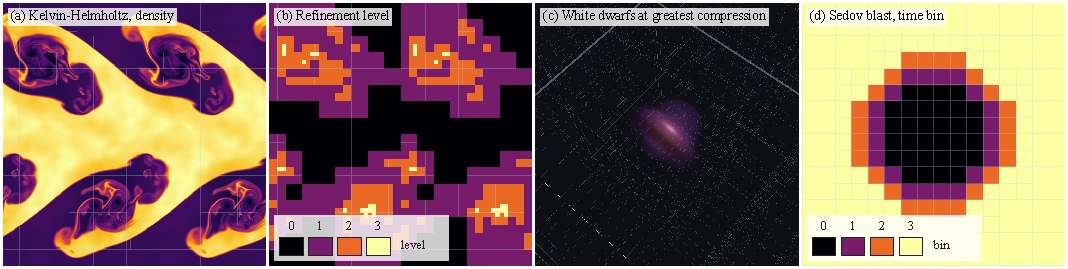
\includegraphics[width=\textwidth]{figures/amr.pdf}
\caption{The adaptive mesh, drawn by the code's own renderer. (a)~Density of a two-dimensional Kelvin-Helmholtz instability at $t = 1.5$, at an effective resolution of $2048^2$ with three levels of refinement; the faint lines outline the blocks of $16^2$ cells. (b)~Refinement level of the same state. (c)~Isosurfaces of the density of two white dwarfs at the greatest compression of a head-on collision, with the outlines of the blocks. (d)~Slice through a three-dimensional Sedov blast (finest resolution 256 cells, three levels) with local timesteps, each block colored by its time bin; a block in bin $k$ steps $2^k$ times the smallest step. The hot gas behind the shock takes the smallest steps, and the cold gas outside it the largest.}
\label{fig:amr}
\end{figure*}

\subsection{Ghost cells computed on load}
\label{sec:ghost}

Because a pass cannot read and write one \texttt{rgba32float} texture, ghost cells cannot be filled in place by copying from neighbors. Shaderous does not fill them. The pass that converts the conserved state to primitive variables computes every texel of a block, ghost or interior, directly from wherever its value lives: the same block, a neighboring block, the image of a cell across a physical boundary, the average of the finer cells that cover it, or an interpolation from a coarser block. There is no separate exchange step, and no ghost cell is ever stale.

\subsection{Matching fluxes across refinement boundaries}
\label{sec:reflux}

The adaptive solvers of \citet{Berger1984} and \citet{Berger1989}, and the GPU codes that follow them \citep{Schive2010, Wang2010}, store the fluxes that the fine side computes on a coarse face and correct the coarse cell afterward. Shaderous extends the gathering of Section~\ref{sec:conservation} across levels instead. At a refinement boundary the coarse cell recomputes the fluxes of the fine faces that cover its face, from the same fine states, with the same arithmetic as the fine cells. Mass, momentum and energy are therefore conserved to round-off without storing any flux. The validation suite checks that the fluxes agree bit for bit between blocks on the same level and to $10^{-6}$ across refinement boundaries.

\subsection{Local timesteps}
\label{sec:timebins}

The subcycling of \citet{Berger1984} lets fine levels take more steps than coarse ones. Shaderous assigns timesteps per block rather than per level, using power-of-two time bins in the manner of particle codes such as GADGET-2 \citep{Springel2005}. Time advances in cycles of up to eight substeps of the smallest step. At the start of a cycle each block is put in a bin from its own signal speed, on the GPU: a block in bin $k$ advances $2^k$ substeps at a time. Relaxation sweeps then enforce three rules: face neighbors are at most one bin apart, a block next to a faster one steps as fast as it, and a block is never slower than a coarser neighbor.

Across a face whose other side steps twice as often, a block takes the other side's fluxes, recomputed from stored states: half when its own step starts and half at its midpoint. A faster block reads a slower neighbor that is part way through a step from that neighbor's half-step prediction. As at refinement boundaries, nothing is stored and conservation holds to round-off. With self-gravity the potential is solved on every block at the end of a cycle. In between, it is solved only on the blocks that finish a step and carried forward elsewhere at the rate at which it last changed.

The extra passes are not free. In three dimensions each block update costs about 10 percent more without gravity and 50 to 70 percent more with it, where every substep also relaxes the potential. Shaderous therefore reads back, every few cycles, the share of block updates that a cycle actually makes, and falls back to a single timestep while that share is above 80 percent (65 percent with gravity). A three-dimensional Sedov blast at a finest resolution of 256 cells with three levels makes 2.2 times fewer block updates with local timesteps and runs 1.9 times faster. An isothermal collapse at the same resolution makes 2.3 times fewer and runs 1.6 times faster. Figure~\ref{fig:amr}d shows how the bins follow a blast.


\section{Gravity, point masses and sinks}
\label{sec:gravity}

\subsection{Poisson solver}
\label{sec:poisson}

The potential is solved every step by geometric multigrid \citep{Brandt1977}, with red-black Gauss-Seidel smoothing, restriction by the average of eight cells, and trilinear prolongation, warm-started from the previous potential. A V-cycle makes two smoothing sweeps before each restriction, two after each prolongation, and eight on the coarsest level of $2^3$ cells. A step runs two V-cycles on the uniform grid. On the adaptive mesh it runs up to three, and the later ones only while they still reduce the residual. Periodic boundaries subtract the mean density from the source. For isolated boundaries a reduction computes the mass and its first and second moments about the box center, and the boundary values of the potential come from the monopole and quadrupole terms,
\begin{equation*}
\Phi_{\rm b} = -G\left[\frac{M}{r} + \frac{Q_{jk}\,s_j s_k}{2r^5}\right], \qquad Q_{jk} = 3S_{jk} - S_{ll}\,\delta_{jk},
\end{equation*}
where $M$ is the mass, $\mathbf{s}$ the position relative to the center of mass, $r = |\mathbf{s}|$, $S_{jk}$ the second moments of the mass about its center, and repeated indices are summed. The dipole term vanishes about the center of mass.

On the adaptive mesh the potential lives on every block, parents included. The density is averaged into the parents, a level's ghost cells come from its neighbors or are interpolated from the level above, and a multigrid cycle runs inside the blocks, at 16, 8, 4, 2 and 1 cells across. The coupling between levels is one-way: a fine level never corrects the coarse potential beneath it. On a uniform sphere the error stays below 0.3 percent with three levels. A new mesh is solved level by level from the coarsest down. During a run all levels relax in the same dispatches, each against the boundary values that its coarser level had at the start of the cycle, so the cost does not grow with the depth of the tree.

\subsection{Coupling to the gas}
\label{sec:coupling}

Gravity enters the update as kick-drift-kick: half a kick with the old potential inside the update pass, and the other half after the new potential is solved. Applying the whole kick after the flux update leaks internal energy from gas in hydrostatic balance and slowly cools a star. The gravitational energy source defaults to a flux form, in which the work on a cell is the mass flux through each face times the difference of the potential across it, as in \citet{Springel2010}. Along one axis, the energy of cell $i$ changes by
\begin{equation*}
\begin{aligned}
\Delta E_i = -\frac{\Delta t}{2\Delta x}\bigl[&F_{i+1/2}\,(\Phi_{i+1} - \Phi_i)\\
&+ F_{i-1/2}\,(\Phi_i - \Phi_{i-1})\bigr],
\end{aligned}
\end{equation*}
where $F$ is the mass flux through a face and $\Phi$ is extrapolated to the half step; the axes add. The work that leaves one cell enters its neighbor, so this conserves total energy. The alternative adds exactly the kinetic energy of each kick, so gravity never touches the internal energy, at the cost of total-energy conservation where the flow is under-resolved. Figure~\ref{fig:gravitytests}a compares the two forms in the collapse of \citet{Evrard1988}. Optionally, a pressure floor keeps the Jeans length resolved by a chosen number of cells, at least the four of \citet{Truelove1997}.

\begin{figure}[t]
\centering
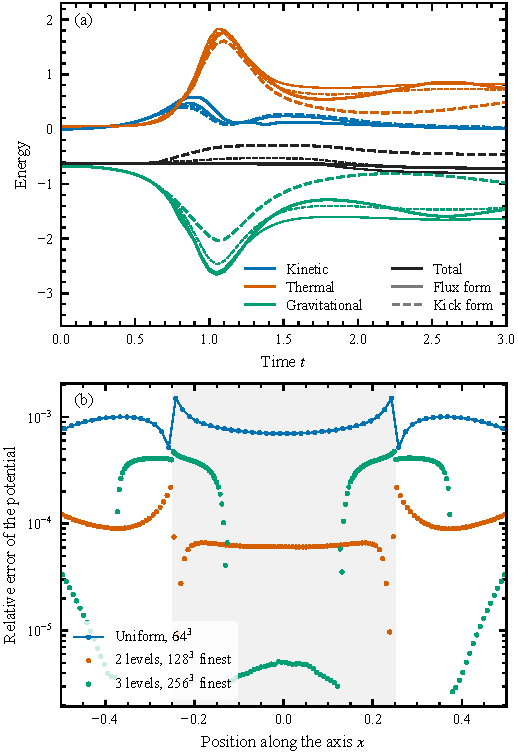
\includegraphics[width=\columnwidth,height=\colfigheight,keepaspectratio]{figures/gravity.pdf}
\caption{Gravity. (a)~Kinetic, thermal, gravitational and total energy during the collapse of \citet{Evrard1988}, with the gravitational energy source in flux form (solid) and kick form (dashed), on a uniform grid of $64^3$ cells (thick lines) and on the adaptive mesh with a finest resolution of 128 cells and two levels (thin lines). After $t \approx 1.5$ the outgoing shock reaches the edge of the box and gas leaves it. (b)~Relative error of the potential of a uniform sphere with isolated boundaries, along the $x$ axis through its center, on a uniform grid and with two and three levels of refinement; the sphere fills the shaded interval.}
\label{fig:gravitytests}
\end{figure}

\subsection{Initial states in discrete balance}
\label{sec:settle}

A star set up from its analytic profile is in balance with the analytic potential, not with the one that the Poisson solver finds on the grid, and it rings in response to the mismatch. As \citet{Zingale2002} do for stellar models mapped onto a grid, Shaderous settles every star of a problem before the first step. The density is set to satisfy $h(\rho) + \Phi = C$ with the grid's potential and the star's mass, where $h$ is the specific enthalpy of the star's cold gas and $C$ a constant, the potential is solved again, and the two are repeated until the density changes by less than $10^{-5}$, which takes six to eight rounds for a polytrope. Several stars settle together, in the same rounds. Each is balanced in its own potential: the grid's potential less the pull of the other stars, which outside a spherical star is that of a point of its mass. A star that moves keeps its velocity. A round changes only the density, and $C$ is found by regula falsi from its value in the previous round. For white dwarfs each round's change is over-relaxed by a factor of 1.6, and the rounds stop at a change of $10^{-3}$. They settle in 7 to 12 rounds, which take 1.6 to 5.5~s at finest resolutions of 256 and 512 cells. Mapped without settling, a white dwarf of one solar mass rang in its fundamental mode, and its central density swung by 30 percent at a finest resolution of 256 cells (Figure~\ref{fig:balance}b). Its core is close to relativistic, with $\Gamma_1$ not far above 4/3, so the small mismatch meets little restoring force. Settled, the central density stays within 0.5 percent over six dynamical times. For a polytrope of index 1 this relation is exactly the trapezoid rule of Equation~(\ref{eq:wb}). On the adaptive mesh, at a finest resolution of 128 cells with two levels, the central density of the settled polytrope strays by 0.14 percent over three dynamical times, against 0.26 percent for the plain scheme, and its energy by 0.33 percent against 0.77 percent.

\subsection{Point masses and sinks}
\label{sec:sinks}

Up to four point masses act on the gas through Plummer-softened gravity \citep{Plummer1911}. They share the gravity field texture with self-gravity, so the hydrodynamic passes do not know that they exist. Each step the masses drift; then one reduction over the updated gas gives every mass its pull on the gas, whose reaction moves the mass, and what its sink takes. The second half-kick pass removes exactly that amount from the cells. Inside a sink radius gas is removed at a rate that falls from $\sqrt{GM/r^3}$ at the center to zero at the radius, and the gas that is removed takes its momentum to the mass. Mass and momentum are conserved between gas and masses to $10^{-7}$ in the validation test. Sinks in grid codes go back to \citet{Bate1995}, \citet{Krumholz2004} and \citet{Federrath2010}; our removal at a local orbital rate is closer to the sinks of circumbinary-disk studies, such as \citet{Farris2014}, who remove gas on a local viscous timescale. The pull between two masses is softened by the larger of their two lengths. By default the softening length and the sink radius of a mass are two cells. On the adaptive mesh these are cells of the finest level when the problem keeps the blocks near its masses at that level, as the binary problem does. Otherwise they are cells of the coarsest level, the only size that the mass is sure to find.

The timestep of the gas does not follow two masses that pass close to one another. Each pair of masses therefore limits the step to one sixteenth of the CFL number times the lesser of $r/v$ and $\sqrt{r^3/GM}$, where $r$ is the softened separation of the pair, $v$ its relative speed and $M$ its total mass. At the default CFL number of 0.8 a circular orbit takes about 125 steps. Two masses on an orbit of eccentricity 0.9 in near-empty gas keep the energy of the orbit to 0.7 percent over two periods with this limit. Without it they lose 94 percent.

The frame is inertial unless a problem asks for another. The tidal disruption problem uses the rest frame of the gas: as in the simulations of \citet{Guillochon2009} and \citet{Guillochon2013}, the frame accelerates with the center of mass of the gas, so the star stays at the box center while the perturber's orbit is integrated alongside the gas. The binary problem uses the rest frame of the masses instead. That frame accelerates with the mean pull of the gas on the masses, and the gas feels the opposite acceleration. After each step we also set the velocity of the masses' center of mass back to zero, which removes the slow drift that rounding in their mutual pull and the momentum of accreted gas would cause. The box, its boundaries and the damping zone of the disk (Section~\ref{sec:interface}) then move with the binary.

\section{Interface, input and output}
\label{sec:interface}

Shaderous runs at a web address. A user picks a problem, a grid and the physics, and watches the gas through a ray-marched volume rendering or an axis-aligned slice, both drawn on the same device from the simulation textures (Figure~\ref{fig:gallery}). The view can show the density, temperature, pressure, a passive scalar, the speed and each velocity component, the Mach number, the entropy function $p/\rho^\gamma$, the net heating rate, the vorticity, the divergence of the velocity, the normalized density gradient $|\nabla\rho|/\rho$, the gravitational potential, the kinetic energy density, the Jeans length in cells and, on the adaptive mesh, the refinement level. The color range follows the field as it evolves, and for the derived fields it ignores the most extreme 0.5 percent of cells. Brushes add mass, velocity or heat; obstacles and sources can be drawn; and the sink tool places point masses. A query tool shows the state of the cell under the pointer and, on the adaptive mesh, the block that holds it, its level and its refinement indicator. The refinement thresholds can be changed during a run. The address bar records the problem, the grid and every setting that differs from the problem's defaults, so a link reproduces a setup.

\begin{figure*}[t]
\centering
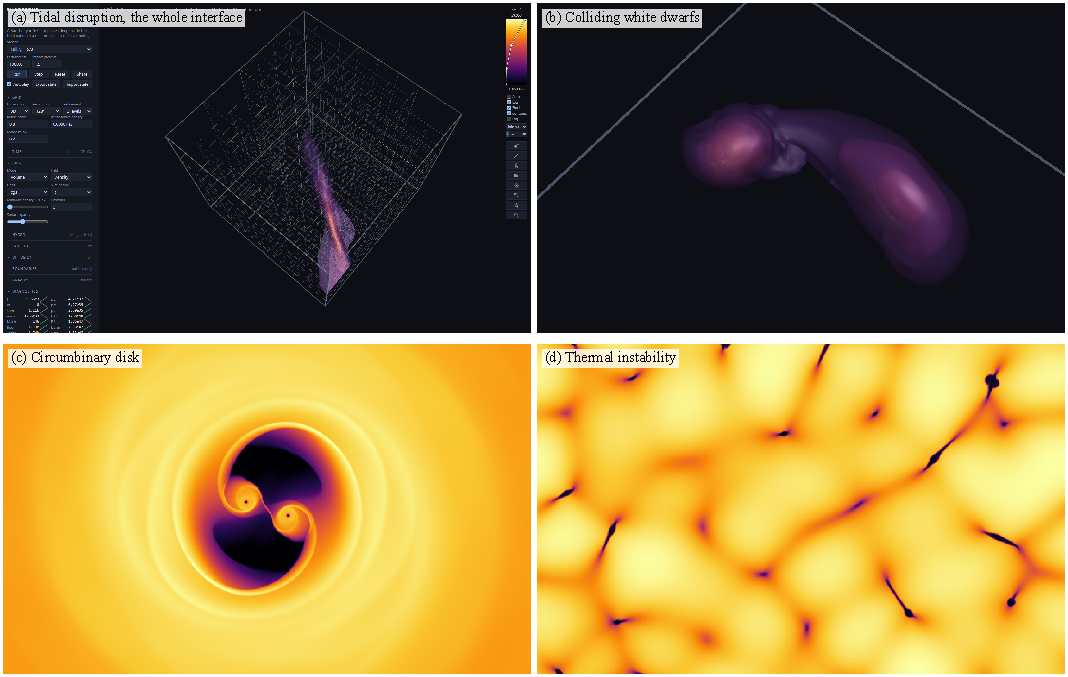
\includegraphics[width=\textwidth]{figures/gallery.pdf}
\caption{Shaderous in the browser. (a)~The whole interface during a three-dimensional tidal disruption on the adaptive mesh ($\beta = 1.5$, $t = 6$), with isosurfaces of the density in the volume view, the problem and physics controls, and the diagnostics. (b)~Isosurfaces of the density of two white dwarfs of 1.0 and $0.8\,\Msun$ after an off-center collision (pericenter 0.6 times the sum of their radii): the lighter one is torn into a tail of debris. (c)~Density of gas around an accreting binary of equal masses after 20 orbits, with the cavity and the streams that cross it. (d)~Temperature in the thermal instability at $t = 0.6$, with cold clouds and filaments (dark) in a warm medium. Every panel was drawn by the code's own renderer; the script that made the figure records each setup as the link that reproduces it.}
\label{fig:gallery}
\end{figure*}

The state can be exported as an HDF5 file in the layout of Athena++ \citep{Stone2020}, which yt reads directly \citep{Turk2011}, in two and three dimensions and on uniform and adaptive grids. Files written by Shaderous also carry the run's settings, time and point masses, so importing one continues the run on the same mesh. Each species is written as a variable named after it. Checkpoints write the same file each time the simulated time passes a multiple of a set interval.

The same page can also run without a person at it. A programming interface in the page loads a setup described by the keys of a link, advances the run by a number of steps or to a given time, and returns diagnostics, samples of the gas, images of the view and exported files as plain data. When the run advances to a given time, its last step is shortened so that it ends at that time exactly. With one parameter in the address, the page neither draws nor plays by itself, so the GPU takes only the steps that a script asks for. Two tools in the repository build on this interface, and both open the page in a browser without a window. A command-line program runs a setup, or a sweep over the values of its parameters. It writes the diagnostics, images, slices and HDF5 files at fixed intervals of simulated time, together with the setup, the version of the code and the GPU that produced them. A server for the Model Context Protocol\footnote{\url{https://modelcontextprotocol.io}} offers the same operations to an AI agent as tools. Within one conversation the agent can load a problem, advance it, read the numbers back and inspect images of the flow.

The problems that ship with the code are the shock tubes of \citet{Sod1978} along each axis and the diagonal and a strong shock tube from \citet{Toro2009}, the blast of \citet{Taylor1950} and \citet{Sedov1959}, Kelvin-Helmholtz and Rayleigh-Taylor instabilities, the Mach 3 wind tunnel with a step of \citet{Emery1968} and \citet{Woodward1984}, smooth advection, the Jeans instability \citep{Jeans1902}, a polytrope of index 1 in equilibrium, a cold white dwarf in equilibrium, two white dwarfs that collide on a parabolic orbit \citep{Rosswog2009, Raskin2009}, the collapse of \citet{Evrard1988}, a uniform sphere, an isothermal turbulent collapse, the thermal instability \citep{Field1965} with the cooling function of \citet{Koyama2002}, a tidal disruption of a polytropic star by a point mass, and a binary accreting from a viscous circumbinary disk \citep{Artymowicz1994, MacFadyen2008}.

Two of these problems use the diffusive fluxes of Section~\ref{sec:diffusion} by default. The disk of the binary has $\nu = 10^{-3}$ in units of the square of the binary's separation times its orbital frequency. At the binary's separation this equals an $\alpha$ viscosity with $\alpha = 0.1$, the value that \citet{Farris2014} chose. The thermal instability has $\kappa = 3 \times 10^{-4}$ in units of the box size and the problem's unit of time, so that conduction rather than the cell size sets the size of the clouds. \citet{Koyama2004} showed that simulations of this instability converge with resolution only if they include conduction and resolve the Field length with at least three cells. With conduction the scale of the structure at $t = 0.6$ changes by 8 percent between $512^2$ and $1024^2$ cells. Without it the scale falls by 20 percent.

The disk of the binary also has a damping zone at its outer edge, of the kind that \citet{deValBorro2006} used to compare codes for disk-planet interaction. Beyond 4.5 binary separations from the center, the density, velocity and specific internal energy of the gas relax toward the initial disk. The rate of relaxation rises from zero there to three times per local orbital period at the edge of the box, 6 separations from the center, and both values can be changed during a run. Without the zone, gas flowed in through the outflow boundaries at the corners of the box, and the disk grew until its uneven pull pushed the binary out of the box. A zone that is fixed to the box brings a second problem. The outer disk then takes up none of the binary's recoil, and a fixed disk pulls an off-center binary further toward its near side. Following the masses' center of mass (Section~\ref{sec:sinks}) removes this instability.

For the tidal disruption the code also sorts the debris by its specific orbital energy about the black hole, from which follows the rate at which bound debris returns to pericenter. Gas that has left the box moves almost ballistically in the potential of the black hole, so its energy no longer changes. The update therefore adds the mass that crosses each open face of the box to a histogram of energy as it crosses. A census adds the gas that is still in the box. It sets apart a surviving core, which we find by iteration: gas belongs to the core if it is bound to the core's mean velocity by the gas's own potential, and the core's mean velocity is then recomputed from that gas. The histograms are sums of 64-bit integers, so they are exact and do not depend on the order in which the GPU adds them. In the validation runs, the mass in the box, the mass that has left and the mass that the sink has taken add up to the starting mass to within the rounding of the total. Kepler's third law turns the histogram of the bound debris into a rate of return (\mbox{Figure~\ref{fig:tde}}). When a star of index 3/2 passes a black hole of $10^6\,\Msun$ at $\beta = 1.5$, the rate peaks at $4.4\,\Msun\,\mathrm{yr}^{-1}$ 37~d after pericenter and then falls close to $t^{-5/3}$. At this resolution a clump of $0.13\,\Msun$ stays bound. At $\beta = 0.6$ the star keeps $0.94\,\Msun$, and the rate falls faster than $t^{-5/3}$, as \citet{Guillochon2013} found for encounters that leave a core.

\begin{figure}[t]
\centering
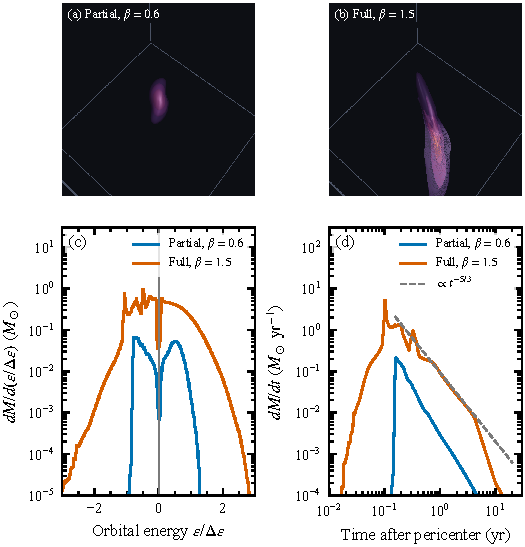
\includegraphics[width=\columnwidth,height=\colfigheight,keepaspectratio]{figures/tde.pdf}
\caption{Tidal disruptions of a polytrope of index 3/2 with the mass and radius of the Sun by a black hole of $10^6\,\Msun$, run with the command-line runner on the adaptive mesh ($128^3$ at the finest level, two levels of refinement). (a, b)~Isosurfaces of the density drawn by the code's renderer at $t = 6$, about two dynamical times after pericenter, five levels evenly spaced in $\log\rho$ from 0.01 to 10~$\Msun\,\Rsun^{-3}$, for impact parameters $\beta = 0.6$ (the star keeps most of its mass) and $\beta = 1.5$ (it is torn apart). (c)~Mass per unit specific orbital energy about the black hole, in units of the spread $\Delta\epsilon = G M_\mathrm{bh} R_\star / r_\mathrm{t}^2$, 20 dynamical times into the run: the gas that has left the box and the gas in it, without the surviving core. (d)~The rate at which the bound debris returns to pericenter, against time since pericenter; the dashed line falls as $t^{-5/3}$. The partial disruption returns its debris in a narrow peak and then falls more steeply.}
\label{fig:tde}
\end{figure}

\section{Educational use}
\label{sec:education}

Several properties make the code practical in a classroom. It needs no installation, no account and no allocation of computing time. It runs on the laptops that students already own, and the two-dimensional problems run on phones. A link records a whole setup, so an instructor can hand a class a prepared run by posting its address. The brushes, the query tool and the choice of displayed field let students change a flow while it runs and read the state of any cell. An exported file opens in yt, so students who know Python can analyze runs with their own scripts. A guide in the repository (\url{https://github.com/guillochon/shaderous/blob/main/docs/teaching.md}) gives each activity below with links that open its setup. \todo{Say whether these activities have been used in a course, and what came of it.}

For undergraduates who are not majoring in physics or astronomy, the code works as a set of demonstrations that need no equations. A Kelvin-Helmholtz instability rolls up into the billows seen in clouds and in the bands of Jupiter. A Rayleigh-Taylor instability grows fingers like the filaments of the Crab Nebula. A Sedov-Taylor blast shows a thin, dense shell around a hot, thin interior, as in a supernova remnant, and opens a discussion of how \citet{Taylor1950} estimated the energy of an explosion from photographs of its fireball. A polytrope at rest shows the balance between pressure and gravity in a star. A tidal disruption, in which students change the depth of the orbit, shows a star torn apart by a black hole. In each, students predict what will happen before they run it.

For physics and astronomy majors the same problems become quantitative. In a shock tube, students identify the rarefaction, the contact discontinuity and the shock, check the jump conditions with the query tool, and compare limiters by editing the link. From dimensional analysis they derive the growth of the Sedov-Taylor radius as $(E t^2/\rho)^{1/5}$ and fit it to a run. They measure the growth rates of the Rayleigh-Taylor and Jeans instabilities and compare them with linear theory. They compare the density profile of the polytrope with the Lane-Emden solution, and turn off the well-balanced reconstruction to see what it does. The thermal instability shows how the cooling curve sets the phases of the interstellar medium, and how conduction sets the size of the smallest clouds. A longer laboratory exercise asks students to run a problem with a known answer at four resolutions, compute the error with yt, and measure the order of convergence, including why shocks converge at first order.

For graduate students the code is a readable example of a modern Godunov method. It has about 6,000 lines of WGSL and 15,000 of TypeScript, and each physical module is a small file. Exercises compare the Riemann solvers on a contact discontinuity and a Gresho vortex, find the carbuncle by turning off the HLL blend at a grid-aligned shock, compare the flux and kick forms of the gravitational energy source in the Evrard collapse, and measure when local timesteps pay for themselves. Term projects include adding a Riemann solver or a test problem with its own validation test, an implicit solver for diffusion, a study of single against double precision using the CPU reference of Section~\ref{sec:validation}, and a performance study from the per-pipeline timing. We pair these with the introduction of \citet{Trac2003} and the texts of \citet{LeVeque2002} and \citet{Toro2009}.

\section{Validation}
\label{sec:validation}

Validation runs in the browser on the reader's own GPU, from a page next to the simulator, and from the command line through a browser driven by Playwright. A double-precision CPU implementation of the same scheme, and an exact Riemann solver \citep{Toro2009}, serve as references. Table~\ref{tab:validation} lists the 36 tests and their pass criteria. Figure~\ref{fig:hydro} compares the hydrodynamics with exact solutions and shows how the error falls with resolution. Figure~\ref{fig:gravitytests} shows the energy budget of a gravitational collapse and the accuracy of the potential on the adaptive mesh. \todo{Add a column with the measured value of each test from a saved run of the suite, and the GPU and browser it ran on.}




\begin{table*}
\centering
\caption{The validation suite. Criteria are those coded in the suite; L1 errors are means over cells, relative to the mean density.}
\label{tab:validation}
\footnotesize
\begin{tabular}{ll}
\toprule
Test & Pass criterion \\
\midrule
Sod tube along $x$, $y$, $z$ & \tabpar{11.4cm}{L1 density error $< 0.01$; runs agree under axis permutation to $10^{-6}$} \\
Sod tube along the diagonal & \tabpar{11.4cm}{L1 density error $< 0.015$} \\
Strong shock tube (pressure ratio $10^5$) & \tabpar{11.4cm}{No floored cells; relative L1 density error $< 0.1$ at 128 cells} \\
Sedov-Taylor blast & \tabpar{11.4cm}{Mean shock radius within 2\% of the similarity solution} \\
Kelvin-Helmholtz & \tabpar{11.4cm}{Transverse kinetic energy grows more than fivefold by $t = 1$} \\
Low-Mach HLLC & \tabpar{11.4cm}{Gresho vortex loses less than half the energy lost with plain HLLC, and gains none} \\
Well-balanced column & \tabpar{11.4cm}{Largest Mach number $< 10^{-4}$ after a sound crossing, at least 100 times below the plain scheme} \\
Uniform advection, 10 crossings & \tabpar{11.4cm}{Mass and momentum drift $< 2 \times 10^{-6}$} \\
Smooth advection & \tabpar{11.4cm}{Mean error $< 2 \times 10^{-4}$ at $256^2$; second order or better} \\
Flux determinism & \tabpar{11.4cm}{Bit-identical mass fluxes on every face, three flows} \\
Blast in a reflecting box & \tabpar{11.4cm}{Mass to $10^{-5}$, total energy to $10^{-3}$} \\
Two-dimensional grids & \tabpar{11.4cm}{Sod L1 error $< 0.003$ at $256^2$; bit-identical fluxes} \\
Rayleigh-Taylor & \tabpar{11.4cm}{At rest, Mach $< 10^{-3}$ at $t = 2$; perturbed, energy to $10^{-3}$} \\
Block grid without refinement & \tabpar{11.4cm}{Identical to the uniform grid, cell by cell} \\
Adaptive Sod tube & \tabpar{11.4cm}{L1 error $< 0.003$ on under 60\% of the cells; mass and energy to $10^{-6}$} \\
Adaptive Sedov blast & \tabpar{11.4cm}{Radius within 2\%; mass and energy to $10^{-6}$} \\
Adaptive instabilities & \tabpar{11.4cm}{Mass to $10^{-6}$, energy to $10^{-5}$ while the mesh follows the flow} \\
Adaptive Poisson solve & \tabpar{11.4cm}{Sphere potential within 1\% with 0, 2 and 3 levels; Jeans rate within 5\%} \\
Adaptive Evrard and polytrope & \tabpar{11.4cm}{Energy to 2\% through bounce; central density within 10\%} \\
Adaptive tidal disruption & \tabpar{11.4cm}{Pericenter within 2\%; frame centered to 0.005 stellar radii} \\
Local timesteps & \tabpar{11.4cm}{Sod and Sedov as with one timestep; mass and energy to $10^{-6}$} \\
HDF5 export and import & \tabpar{11.4cm}{Restarted state equal to $10^{-5}$; continued runs agree to $10^{-4}$} \\
Cooling & \tabpar{11.4cm}{Power-law decay to 0.1\%; thermal balance to 1\% without overshoot} \\
Viscosity & \tabpar{11.4cm}{Energy of a shear wave decays as $\exp(-2\nu k^2 t)$ to 1\%, and to 3\% between no-slip walls; energy to $10^{-5}$ on the adaptive mesh} \\
Conduction & \tabpar{11.4cm}{Temperature wave decays at the linear rate to 1\%; cloud scale of the thermal instability changes by $< 12\%$ when the resolution doubles} \\
Point mass and sink & \tabpar{11.4cm}{Gas plus accreted mass constant to $10^{-5}$} \\
Binary orbit & \tabpar{11.4cm}{Separation within 0.5\% over one period; both masses accrete} \\
Close encounter of two masses & \tabpar{11.4cm}{Orbit of eccentricity 0.9 keeps its energy to 1\% over two periods} \\
GPU against CPU reference & \tabpar{11.4cm}{Density and energy differ by $< 10^{-4}$ of the mean after 20 steps} \\
Equations of state & \tabpar{11.4cm}{Round trip to $10^{-5}$; WGSL matches float64 mirrors to $10^{-4}$, degenerate electrons and hydrogen ionization included} \\
Uniform sphere potential & \tabpar{11.4cm}{Largest error $< 1\%$ (isolated boundaries)} \\
Jeans instability & \tabpar{11.4cm}{Growth rate within 5\% of linear theory} \\
Polytrope & \tabpar{11.4cm}{Central density within 10\% over 10 dynamical times} \\
Cold white dwarf & \tabpar{11.4cm}{Settled $0.6\,M_\odot$ dwarf: central density within 5\% over three dynamical times; energy to $10^{-3}$} \\
Evrard collapse & \tabpar{11.4cm}{Total energy to 2\%; thermal energy peaks at $0.9 < t < 1.3$} \\
Tidal disruption & \tabpar{11.4cm}{Pericenter within 2\%; star disrupted} \\
\bottomrule
\end{tabular}
\end{table*}

\section{Performance}
\label{sec:performance}

The flux update is limited by texture fetches rather than arithmetic, which is why the uniform grid stores no primitive variables. In two dimensions a run uses $16 \times 16 \times 1$ workgroups, which more than halves the cost of the flux update against $8 \times 8 \times 4$ workgroups with three idle layers. The number of steps per frame adapts to the GPU, and results agree across browsers to round-off. On the adaptive mesh the passes that cover a block and its ghost layers, 18 or 20 cells across, run as rows of 64 threads per block, because $8 \times 8 \times 4$ tiles left about half of their threads idle there. In two dimensions the four layers of a workgroup take four blocks. These two changes made a step of a two-dimensional Kelvin-Helmholtz problem 2.8 times faster, and a step of a three-dimensional Sedov blast 19 percent faster. The interface can also report the GPU time that each pipeline takes, from timestamp queries. Figure~\ref{fig:performance} shows the throughput on a discrete GPU in Chrome, measured with the scripting interface at normal priority. A uniform grid of $2048^2$ cells takes $1.3 \times 10^9$ cell updates per second, and one of $256^3$ cells $9.3 \times 10^8$. On the adaptive mesh a leaf cell costs more than a cell of a uniform grid, because its ghost cells are computed as they are loaded and the refinement boundaries recompute fine fluxes. In two dimensions the mesh still takes $5.5$ to $6.8 \times 10^8$ updates per second, and in three, $5.2$ to $5.4 \times 10^8$ with two and three levels. With four levels, a three-dimensional blast early in its expansion takes only $5.9 \times 10^7$ \todo{Find out why: the mesh changes every few steps then, and each level adds passes.} \todo{Measure an integrated GPU and Firefox, and compare with a published throughput of a CUDA code on similar hardware.}

\begin{figure}[t]
\centering
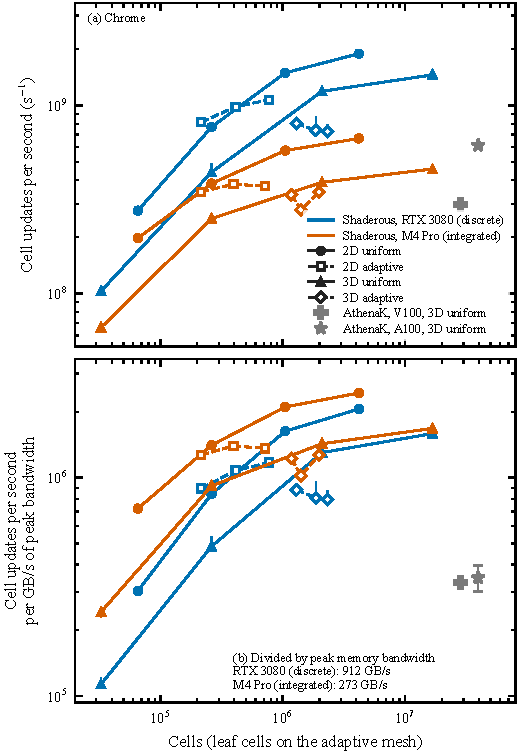
\includegraphics[width=\columnwidth,height=\colfigheight,keepaspectratio]{figures/performance.pdf}
\caption{Throughput on one discrete GPU (NVIDIA, Ampere generation) in Chrome. Cell updates per second against the number of cells, for a two-dimensional Kelvin-Helmholtz instability and a three-dimensional Sedov blast, each on uniform grids and on adaptive meshes (one to four levels, local timesteps off). On the adaptive mesh every leaf cell counts as one update per step. \todo{Add an integrated GPU and Firefox, and a published throughput of a CUDA code on similar hardware.}}
\label{fig:performance}
\end{figure}

\section{Discussion}
\label{sec:discussion}

Shaderous is not a replacement for production codes. It runs on one GPU, its memory is bounded by what the browser will allocate (in three dimensions the adaptive mesh holds at most 2197 blocks, about 3~GB with gravity), and it has no magnetic fields or radiation transport. Its viscosity and conduction are explicit and have constant coefficients. Single precision is adequate for the problems that ship with the code, but round-off is biased when a uniform background sits exactly on a power of two, and long integrations accumulate errors that double precision would not.

The design choices of Sections~\ref{sec:conservation} to~\ref{sec:amr} came from constraints of WebGPU, but they do not depend on it. Gathering fluxes and recomputing them across refinement and time-bin boundaries trades extra arithmetic for less storage and less memory traffic, which suits any processor whose throughput is limited by memory rather than by arithmetic. Computing ghost cells on load removes a synchronization step from every AMR cycle.

We are developing a nuclear burning module for the white dwarf problems, and the species of Section~\ref{sec:species} are laid out so that it can take over their state. A small neural network is being trained to step the 13-isotope $\alpha$-chain network of \citet{Timmes2000}, which we build with pynucastro \citep{SmithClark2023}, at constant density with the heat that the burning releases. The network predicts the new mass fractions through a softmax, so that they stay positive and sum to one. The energy released follows from the change in composition and is not predicted. The states that the network reaches when it is applied step after step are labeled with the reference network and added to its training set, following the DAgger method of \citet{Ross2011}.

\section{Conclusions}
\label{sec:conclusions}

Shaderous is a compressible hydrodynamics code with self-gravity, adaptive mesh refinement, local timesteps, point masses, sinks, cooling, viscosity and conduction, written entirely in WebGPU compute shaders and run from a web page. It conserves mass, momentum and energy to round-off on its adaptive mesh without storing any face flux, by having every cell recompute the fluxes it needs, bit for bit, across refinement and time-bin boundaries. It keeps every step on the GPU and computes ghost cells as it loads them. It works in single precision and holds hydrostatic stars and atmospheres in balance through a well-balanced reconstruction and a settled initial state. The code and its validation suite run on the reader's own GPU, and a link reproduces any setup. Scripts and AI agents can drive the same page without a person at it. The same properties make it a tool for teaching, from demonstrations for non-major undergraduates to term projects for graduate students.

\begin{acknowledgments}
We thank J. Xavier Prochaska for providing access to the Claude team through which all of the Claude models named below were used.

The code, its validation suite, the manuscript source, the bibliography and the notes behind every number in the text are available online.\footnote{\url{https://github.com/guillochon/shaderous}} The author takes full responsibility for the contents of this paper and of the code. Large language models (Claude Opus 5.5 and Claude Fable 5.2) were used, under author supervision, to write and test the code, to search the literature, to draft and edit the text and the online documentation, and to measure the numbers that the text quotes. Every number in the text is traced to the code, to a measurement recorded in the repository, or to a cited paper. Every bibliography entry was checked against the NASA Astrophysics Data System, Crossref or arXiv, and all references and AI edits were hand-checked by the author. We aimed to be compliant with the AAS guidelines on generative AI in manuscript preparation.\footnote{\url{https://journals.aas.org/author-llm-guidelines}} Those guidelines do not treat such tools as authors; responsibility for accuracy remains with the listed author.
\end{acknowledgments}

\software{Shaderous (\url{https://github.com/guillochon/shaderous}), TypeScript, Vite, Vitest, Playwright, h5wasm, yt \citep{Turk2011}}

%% ---- END BODY ----

\bibliographystyle{aasjournalv7}
\bibliography{references}

\end{document}
